\section{System Model}
\label{sec:sysmod}

\begin{figure}
\centering
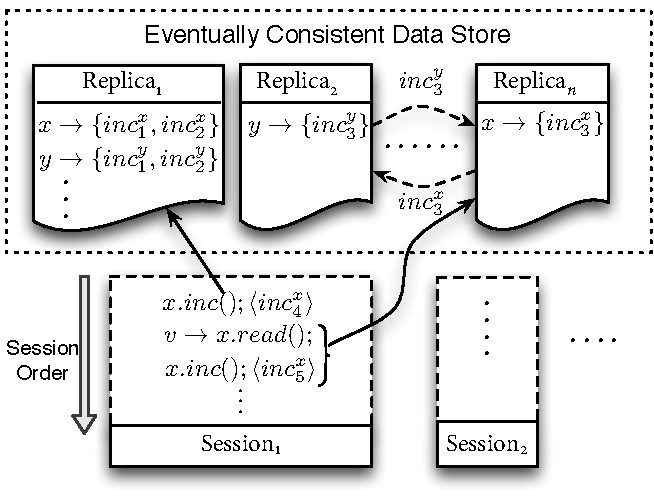
\includegraphics[scale=0.9]{Figures/SystemModel}
\caption{\name system model.}
\label{fig:sysmod}
\end{figure}

Figure~\ref{fig:sysmod} summarizes the abstract system model of a data
store exposed to the \name programmer. The store is a collection of
\emph{replicas}, each storing a set of \emph{objects} ($x,y,\ldots$)
of a replicated data type. For the sake of an example,  let $x$ and
$y$ represent objects of an \emph{increment-only counter} replicated
data type (RDT) that admits \emph{inc} and \emph{read} operations. The
state of an RDT object is represented as the set of all updates
(effectful operations, or simply \emph{effects}) performed on the
object. In Fig.~\ref{fig:sysmod}, the state of $x$ at replica 1 is the
set $\{inc^x_1,inc^x_2\}$, where each $inc^x_i$ denotes an \emph{inc}
effect on $x$.

Clients interact with the data store via concurrent \emph{sessions},
where each session is a sequence of operations that a client invokes
on any of the objects contained in the store. Note that clients have
no control over which replica an operation is applied to; the data
store may choose to route the operation to any replica in order to
minimize latency, load balance, etc. For example, the \emph{inc} and
\emph{read} operations invoked by the same session on the same object,
may be applied on different replicas because replica 1 (to which the
\emph{inc} operation is applied, say) might be unreachable when the
client invokes a subsequent \emph{read}.

When an operation is applied to a replica, it is said to witness the
state of its object at that replica.  For example, \emph{x.inc}
applied to replica 1 witnesses the state of $x$ as
$\{inc^x_1,inc^x_2\}$.  We say that the effects $inc^x_1$ and
$inc^x_2$ are \emph{visible} to the effect ($inc^x_4$) of
\emph{x.inc}, written logically as $\small \vis{inc^x_1}{inc^x_4}
\wedge \vis{inc^x_2}{inc^x_4}$, where $\small \visZ$ stands for the
irreflexive and asymmetric visibility relation between effects over
the same object. The notion of visibility is important since the
result of an operation often depends on the set of visible
effects\footnote{We abuse the visibility relation by informally
  extending it to operations (including read-only operations, which
  produce no effects).}. For instance, a \emph{read} on $x$ applied to
the last replica in Fig.~\ref{fig:sysmod} returns 1 since it only
witnesses the effect ($inc^x_3$) of a single \emph{x.inc} operation.

A visibility relation between two effects implies that the former
operation has happened before the latter (since the latter has
witnessed the effect of the former). However, visibility is not enough
to capture a happens-before order between operations, necessary to
enforce causal consistency. As Fig.~\ref{fig:sysmod} demonstrates, a
pair of operations from the same session, although one happens before
the other, need not be visible to each other. To capture
happens-before, we define an irreflexive transitive \emph{session
  order} relation that relates the effects of operations arising from
the same session. For example, in Fig.~\ref{fig:sysmod}, $inc^x_4$ and
$inc^x_5$ are in session order (written logically as $\small
\so{inc^x_4}{inc^x_5}$).

The effect added to a particular replica is asynchronously sent to
other replicas, and eventually merged into all other replicas. Observe
that this model is independent of the resolution strategy for
concurrent conflicting updates, and instead preserves \emph{every}
update. Update conflicts are resolved when an operation reduces over
the set of effects on an object at a particular replica. The model,
however, admits all the inconsistencies associated with eventual
consistency, some of which could adversely impact the usability of the
application. We call such unacceptable inconsistencies as
\emph{anomalies}. Stronger consistency guarantees are needed to
prevent unwanted anomalies.

In the next section we concretize, in \name, the \emph{counter}
application described informally above, followed by the anomalies the
application admits under our model.  Next, we show that strengthening
the model with a few simple guarantees is enough to prevent these
anomalies. We introduce a specification language that lets us
naturally express such additional requirements. Finally, we show that
well-known high-level consistency guarantees have precise semantics
under our model, and hence can be expressed as formulas in our
specification language. This makes it straightforward to compare
application requirements with consistency guarantees, and determine
the appropriate consistency semantics required to prevent anomalies.

% Bank account is a bad example. We have to explicitly transalate bal
% >= 0 invariant into axiomatic invariants. Counter is a better
% example since it's invariants can be expressed naturally in Quelea.
% It is also more representative of EC web applications.
